\documentclass[11pt]{article}
\usepackage{fullpage,url}
\usepackage{amsmath,amsthm,amssymb}
\usepackage{graphicx}
\usepackage{eso-pic}
\usepackage{bm}
\usepackage{caption}
\usepackage{picins}   
\usepackage{microtype}
%\usepackage{multirow}
\usepackage{url}
\usepackage{enumerate}
\usepackage{pdfpages}
\usepackage{hyperref}
\usepackage[letterpaper,top=1in,bottom=1in,left=1in,right=1in,nohead]{geometry}

\newcommand{\PhiB}{\mathbf{\Phi}}
\newcommand{\Ll}{\mathcal{L}}
\newcommand{\Nn}{\mathcal{N}}
\newcommand{\Uu}{\mathcal{U}}
\newcommand{\Ee}{\mathcal{E}}
\newcommand{\Aa}{\mathcal{A}}
\newcommand{\Hh}{\mathcal{H}}
\newcommand{\Ii}{\mathcal{I}}
\newcommand{\Ff}{\mathcal{F}}
\newcommand{\Dd}{\mathcal{D}}
\newcommand{\Tt}{\mathcal{T}}
\newcommand{\Pp}{\mathcal{P}}
\newcommand{\Ss}{\mathcal{S}}
\newcommand{\Cc}{\mathcal{C}}
\newcommand{\Oo}{\mathcal{O}}
\newcommand{\Bb}{\mathcal{B}}
\newcommand{\Rr}{\mathcal{R}}
\newcommand{\Rm}{\mathrm{R}}
\newcommand{\CB}{\mathbf{C}}
\newcommand{\RB}{\mathbf{R}}
\newcommand{\xB}{\mathbf{x}}
\newcommand{\yB}{\mathbf{y}}
\newcommand{\XB}{\mathbf{X}}
\newcommand{\YB}{\mathbf{Y}}
\newcommand{\fB}{\mathbf{f}}
\newcommand{\tB}{\mathbf{t}}
\newcommand{\ZB}{\mathbf{Z}}
\newcommand{\SB}{\mathbf{S}}
\newcommand{\AB}{\mathbf{A}}
\newcommand{\WB}{\mathbf{W}}
\newcommand{\TB}{\mathbf{T}}

\newcommand{\omitme}[1]{}
\newtheorem*{lemma}{Lemma}
\newtheorem{case}{Case}

\makeatletter
\newcommand{\specialnumber}[1]{%
  \def\tagform@##1{\maketag@@@{(\ignorespaces##1\unskip\@@italiccorr#1)}}%
}

\setlength{\parindent}{0in}
\setlength{\parskip}{6pt}

\DeclareMathOperator{\E}{E}
\DeclareMathOperator{\Var}{Var}
\DeclareMathOperator{\Unif}{Unif}

\begin{document}
\thispagestyle{empty}
{\large{\bf CS6320: 3D Computer Vision \hfill Prateep Mukherjee(u0876583)}}\\

{\LARGE{\bf Homework 2}}
\vspace{0.2\baselineskip}
\hrule


  \vspace{-10pt}
\section{Theoretical Problems}
    \vspace{-10pt}
\subsection{Problem 1}

For 3 cameras, point-to-point correspondence are no longer uniquely defined.  Let us define $u_1, u_2$ and $u_3$ be the 3 images generated using the cameras $c_1,c_2$ and $c_3$ respectively. For uncalibrated cameras, we get the following 3 epipolar equations:
\vspace{-10pt}
\begin{eqnarray}
  u_1^{T} \Ff u_2 = 0 \label{eq1} \\
  u_2^{T} \Ff u_3 = 0 \label{eq2}  \\
  u_3^{T} \Ff u_1 = 0 \label{eq3}
\end{eqnarray}

Therefore, correspondence points for every point($\Re^2$) in $u_1$ are given by two equations $\Ff u_2 = 0$ and $u_3^{T} \Ff = 0$.  This is an over-determined system of linear equations which yields incoherent results. 

\subsection{Problem 2}

\begin{itemize}
  \item For forward translating cameras, the epipoles $e$ and $e'$ have the same coordinates in both the images. Since, all epipolar lines pass through epipoles, therefore the epipolar lines radiate from each epipole. Therefore, correspondence points move along these radiating lines from $e$. This is why we see a radially oriented intersecting planes. 
  \item Given the disparity of the two images, depth-map $\mathbf{Z}$ can be computed by $\mathbf{Z} =- \frac{f \mathbf{B}}{d}$, where $f$ is the focal length of the camera, $\Bb$ is the baseline shift and $d$ is the disparity at a pixel $x$. For forward translating cameras, point $\xB'$ on one camera maps to $\xB$ on the other, such that 
\begin{equation*}
 \xB' = \xB +  \frac{K \tB}{z}
\end{equation*}
where $K$ is the calibration matrix with constant intrinsic and extrinsic parameters. Disparity $d = \xB' - \xB$.  Therefore, the depth of world points can be computed as:
\begin{equation*}
  \mathbf{Z} = - \frac{f\tB}{d} = -\frac{f \tB}{ \frac{K \tB}{z}} = - C.z
\end{equation*}
\end{itemize}

   \vspace{-10pt}
\section{Practical Problems}
    \vspace{-10pt}
\subsection{Problem 4a}
    \vspace{-10pt}
\par Fig \ref{fig1} shows the 2 rectified stereo images used for my experiment.  They are captured with two positions of the camera. Firstly an image( Fig. \ref{fig1}a) is taken. Then, I translate for some distance to the left to take the second image(Fig. \ref{fig1}b). 

\begin{figure}[!hbt]
\vspace{-10pt}
 \begin{center}
  \[ \begin{array}{cc}
	  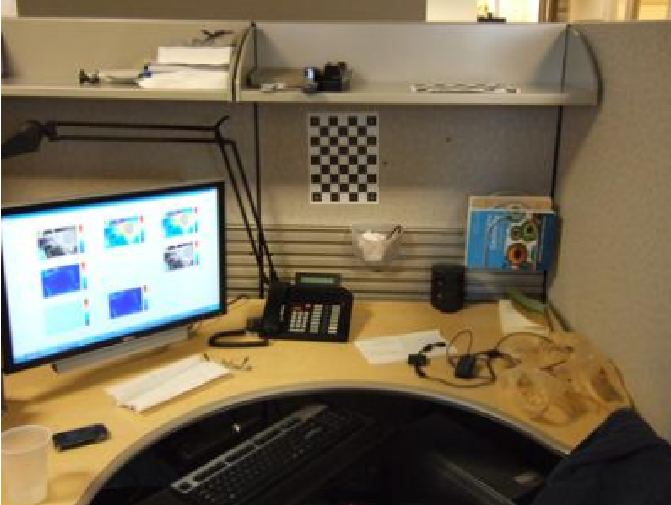
\includegraphics[width=0.5 \linewidth]{deskLeft.png} &
	  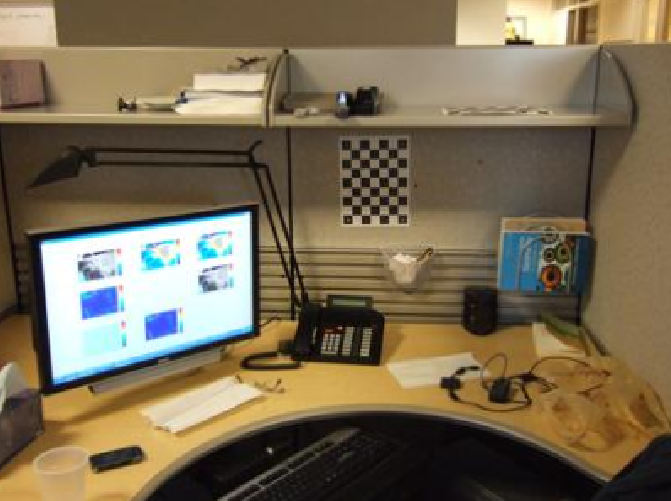
\includegraphics[width=0.5\linewidth]{deskRight.png} \\
	  (a) & (b) \\
	  \end{array} \]
  \end{center}
  \vspace{-10pt}
  \caption{ Image of a desk space captured from two positions of the camera. {\bf (a)} Right view; {\bf (b)} Left view. }
  \label{fig1}
    \vspace{-10pt}
\end{figure}

\par Next, I generate matching points on both the images.  These points were all picked manually. Fig. \ref{fig2} shows the colored points on both images.
    \vspace{-10pt}
\begin{figure}[!hbt]
\vspace{-10pt}
 \begin{center}
  \[ \begin{array}{cc}
	  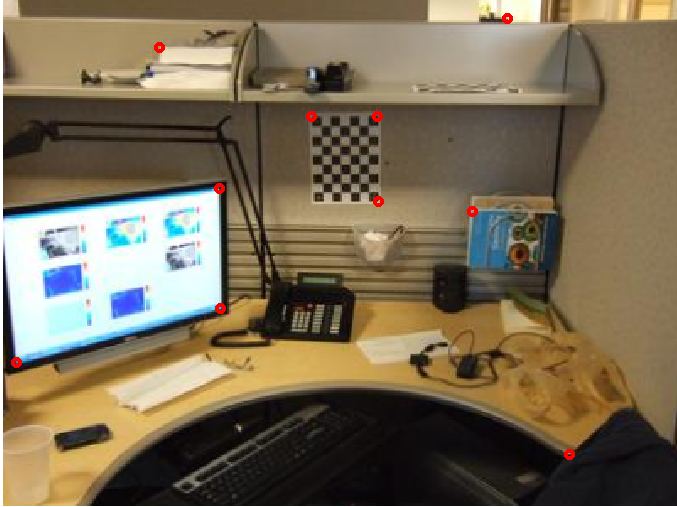
\includegraphics[width=0.5 \linewidth]{deskLeft_pts.png} &
	  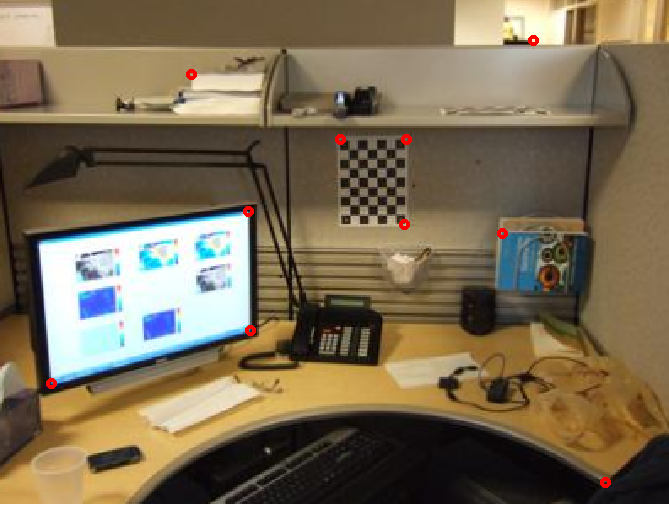
\includegraphics[width=0.5\linewidth]{deskRight_pts.png} \\
	  (a) & (b) \\
	  \end{array} \]
  \end{center}
      \vspace{-10pt}
  \caption{ Images in Fig. \ref{fig1} overlayed with matching points(in red).  A total of 10 points were selected. }
  \label{fig2}
      \vspace{-10pt}
\end{figure}


\par The fundamental matrix $\Ff$ is built from these points.  Since $\Ff$ has only 8 free parameters(setting $\Ff_{33} = 1$), we need only 8 of the above points.  A random sampling is done to pick 8 points in this assignment. A cross-validation study amongst all picked points to pick the ``best'' 8 points can be done, which would give the best epipolar lines. The remaining points on one image are used to compute the epipolar lines on the other.  Fig. \ref{fig3} shows the different experiments with the remaining points on left and right images. 

\begin{figure}[!hbt]
\vspace{-10pt}
 \begin{center}
	  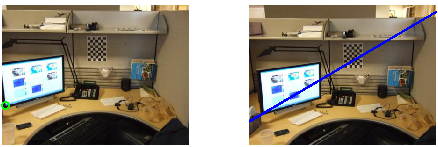
\includegraphics[width=\linewidth]{pic1.png} \\
	  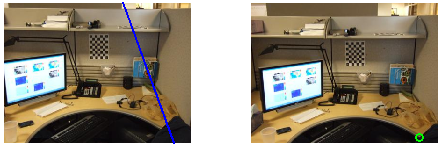
\includegraphics[width=\linewidth]{pic3.png}
  \end{center}
      \vspace{-10pt}
  \caption{ The image pair shown with points(in green) and epipolar line(in blue) . {\bf Top} Epipolar line drawn on right image for corresponding point on left. {\bf Bottom} Epipolar line drawn on left image for corresponding point on right. }
  \label{fig3}
      \vspace{-10pt}
\end{figure}

\par Fig. \ref{fig3} shows that the epipolar lines do pass through corresponding points. 

In order to compute the epipole of the left camera, eigen vector of $\Ff$ is considered which lies in its null-space. Therefore, we seek $u$ such that $\Ff u = \bar{0}$.  This is done by considering the eigen decompostion for $\Ff' \times \Ff$. Then, I taken the eigen vector with the smallest eigen value, and normalize it to get the pixel coordinates of the epipole in homogenous coordinates.  The epipole for the left image is computed at $(250.47,117.22)$. Fig. \ref{fig4} shows the epipole on the left image.

\begin{figure}[t]
  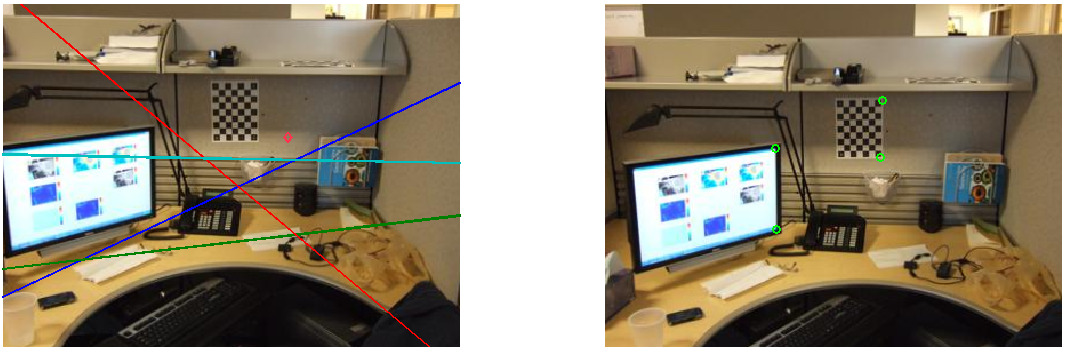
\includegraphics[width=\linewidth]{epipoles.png}
  \caption{Epipole on the left images shown as diamond. }
  \label{fig4}
\end{figure}

\subsection{Problem 4b}
  
    \par I take the classical {\b tsukuba} image from middlebury dataset for my disparity map experiment. Fig. \ref{fig5} shows the pair of images used. The calibration details of the camera is provided at \href{http://vision.middlebury.edu/stereo/data/scenes2014/datasets/Adirondack-perfect/calib.txt}{here}. The original images($2880 \times 1988$) are scaled down to $384 \times 288$ resolution for ease of computation.
    
 \begin{figure}[!hbt]
\vspace{-10pt}
 \begin{center}
  \[ \begin{array}{ccc}
	  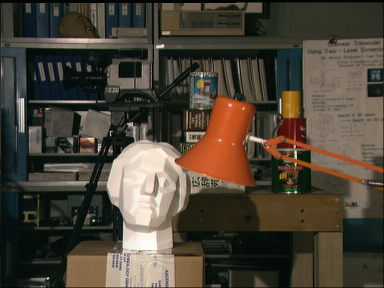
\includegraphics[width=0.33\linewidth]{tsuL.png} &
	  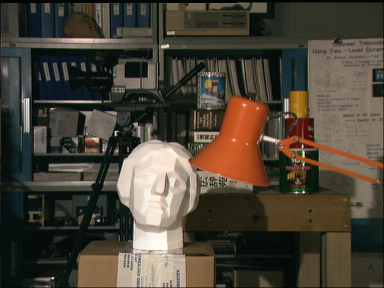
\includegraphics[width=0.33\linewidth]{tsuR.png} & 
	  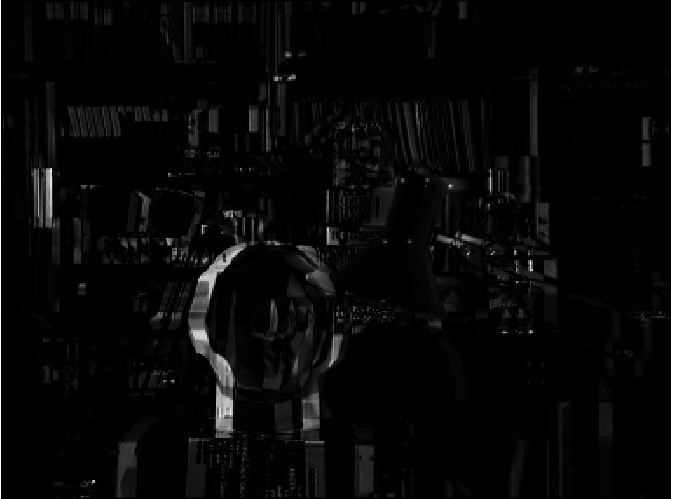
\includegraphics[width=0.33\linewidth]{tsu_diff.png} \\
	  (a) & (b) & (c) \\
	  \end{array} \]
  \end{center}
  \vspace{-10pt}
  \caption{(a,b) : {\bf Tsukuba} stereo images from middlebury vision dataset; (c) Difference image where bright regions show the shift. }
  \label{fig5}
    \vspace{-10pt}
\end{figure}

 \par As input parameter to my code, I get user-specified values for \emph{window\_size}, which is used as region of interest for computing normalized cross-correlation(NCC). Thereafter, I shift the left image and compute NCC for every window patch. The minimum value of NCC is chosen as the value for every pixel. I do this for the other image as well. 
 \vspace{-10pt}
 \begin{figure}[!hbt]
\vspace{-10pt}
 \begin{center}
  \[ \begin{array}{ccc}
	  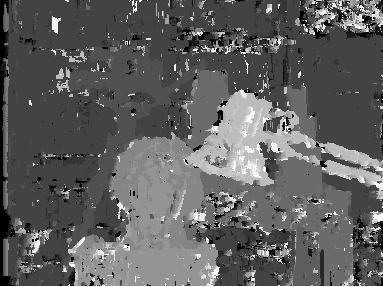
\includegraphics[width=0.33\linewidth]{tsuL_disp.png} &
	  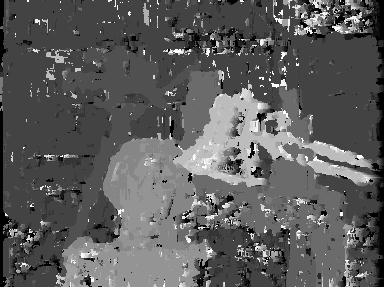
\includegraphics[width=0.33\linewidth]{tsuR_disp.png} \\ 
	  (a) & (b) \\
	  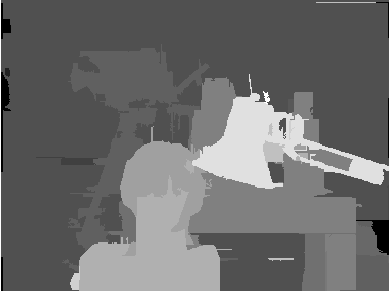
\includegraphics[width=0.33\linewidth]{disp.png} &
	  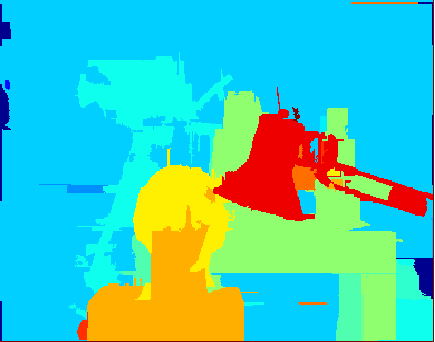
\includegraphics[width=0.33\linewidth]{disp_rgb.png} \\
	  (c) & (d) 
	  \end{array} \]
  \end{center}
  \vspace{-10pt}
  \caption{ Disparity maps for {\bf (a)} left and {\bf (b)} right images. {\bf (c)} Final disparity using the \textbf{winner takes all} strategy. {\bf (d)} Disparity map in rgb.}
  \label{fig6}
    \vspace{-10pt}
\end{figure}

\par Finally, in order to get a good disparity image, I adopt a \textbf{winner takes all} strategy. For every pixel, I compute the minimum disparity from left and right images, and label each pixel with this disparity. Fig. \ref{fig6} shows the disparity maps for left and right  images.

\begin{figure}[!hbt]
\vspace{-10pt}
  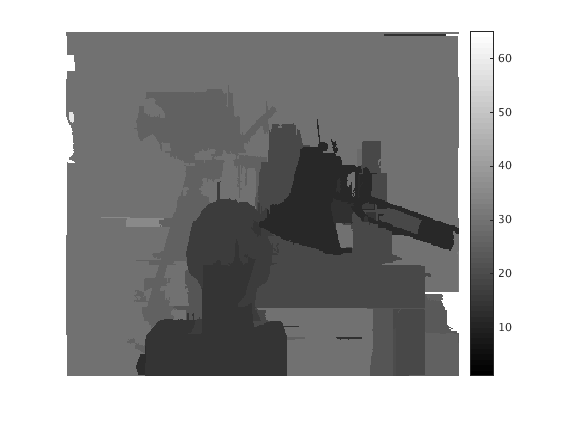
\includegraphics[width=\linewidth]{disp_Z.png}
  \caption{Z-depth shown with baseline shift = 176.252. Lighter regions represent far-away.}
  \vspace{-10pt}
  \label{fig7}
\end{figure}
 
 
\end{document}